% Options for packages loaded elsewhere
\PassOptionsToPackage{unicode}{hyperref}
\PassOptionsToPackage{hyphens}{url}
\PassOptionsToPackage{dvipsnames,svgnames,x11names}{xcolor}
%
\documentclass[
  letterpaper,
  DIV=11,
  numbers=noendperiod]{scrartcl}

\usepackage{amsmath,amssymb}
\usepackage{iftex}
\ifPDFTeX
  \usepackage[T1]{fontenc}
  \usepackage[utf8]{inputenc}
  \usepackage{textcomp} % provide euro and other symbols
\else % if luatex or xetex
  \usepackage{unicode-math}
  \defaultfontfeatures{Scale=MatchLowercase}
  \defaultfontfeatures[\rmfamily]{Ligatures=TeX,Scale=1}
\fi
\usepackage{lmodern}
\ifPDFTeX\else  
    % xetex/luatex font selection
\fi
% Use upquote if available, for straight quotes in verbatim environments
\IfFileExists{upquote.sty}{\usepackage{upquote}}{}
\IfFileExists{microtype.sty}{% use microtype if available
  \usepackage[]{microtype}
  \UseMicrotypeSet[protrusion]{basicmath} % disable protrusion for tt fonts
}{}
\makeatletter
\@ifundefined{KOMAClassName}{% if non-KOMA class
  \IfFileExists{parskip.sty}{%
    \usepackage{parskip}
  }{% else
    \setlength{\parindent}{0pt}
    \setlength{\parskip}{6pt plus 2pt minus 1pt}}
}{% if KOMA class
  \KOMAoptions{parskip=half}}
\makeatother
\usepackage{xcolor}
\setlength{\emergencystretch}{3em} % prevent overfull lines
\setcounter{secnumdepth}{-\maxdimen} % remove section numbering
% Make \paragraph and \subparagraph free-standing
\makeatletter
\ifx\paragraph\undefined\else
  \let\oldparagraph\paragraph
  \renewcommand{\paragraph}{
    \@ifstar
      \xxxParagraphStar
      \xxxParagraphNoStar
  }
  \newcommand{\xxxParagraphStar}[1]{\oldparagraph*{#1}\mbox{}}
  \newcommand{\xxxParagraphNoStar}[1]{\oldparagraph{#1}\mbox{}}
\fi
\ifx\subparagraph\undefined\else
  \let\oldsubparagraph\subparagraph
  \renewcommand{\subparagraph}{
    \@ifstar
      \xxxSubParagraphStar
      \xxxSubParagraphNoStar
  }
  \newcommand{\xxxSubParagraphStar}[1]{\oldsubparagraph*{#1}\mbox{}}
  \newcommand{\xxxSubParagraphNoStar}[1]{\oldsubparagraph{#1}\mbox{}}
\fi
\makeatother


\providecommand{\tightlist}{%
  \setlength{\itemsep}{0pt}\setlength{\parskip}{0pt}}\usepackage{longtable,booktabs,array}
\usepackage{calc} % for calculating minipage widths
% Correct order of tables after \paragraph or \subparagraph
\usepackage{etoolbox}
\makeatletter
\patchcmd\longtable{\par}{\if@noskipsec\mbox{}\fi\par}{}{}
\makeatother
% Allow footnotes in longtable head/foot
\IfFileExists{footnotehyper.sty}{\usepackage{footnotehyper}}{\usepackage{footnote}}
\makesavenoteenv{longtable}
\usepackage{graphicx}
\makeatletter
\def\maxwidth{\ifdim\Gin@nat@width>\linewidth\linewidth\else\Gin@nat@width\fi}
\def\maxheight{\ifdim\Gin@nat@height>\textheight\textheight\else\Gin@nat@height\fi}
\makeatother
% Scale images if necessary, so that they will not overflow the page
% margins by default, and it is still possible to overwrite the defaults
% using explicit options in \includegraphics[width, height, ...]{}
\setkeys{Gin}{width=\maxwidth,height=\maxheight,keepaspectratio}
% Set default figure placement to htbp
\makeatletter
\def\fps@figure{htbp}
\makeatother

\KOMAoption{captions}{tableheading}
\makeatletter
\@ifpackageloaded{caption}{}{\usepackage{caption}}
\AtBeginDocument{%
\ifdefined\contentsname
  \renewcommand*\contentsname{Table of contents}
\else
  \newcommand\contentsname{Table of contents}
\fi
\ifdefined\listfigurename
  \renewcommand*\listfigurename{List of Figures}
\else
  \newcommand\listfigurename{List of Figures}
\fi
\ifdefined\listtablename
  \renewcommand*\listtablename{List of Tables}
\else
  \newcommand\listtablename{List of Tables}
\fi
\ifdefined\figurename
  \renewcommand*\figurename{Figure}
\else
  \newcommand\figurename{Figure}
\fi
\ifdefined\tablename
  \renewcommand*\tablename{Table}
\else
  \newcommand\tablename{Table}
\fi
}
\@ifpackageloaded{float}{}{\usepackage{float}}
\floatstyle{ruled}
\@ifundefined{c@chapter}{\newfloat{codelisting}{h}{lop}}{\newfloat{codelisting}{h}{lop}[chapter]}
\floatname{codelisting}{Listing}
\newcommand*\listoflistings{\listof{codelisting}{List of Listings}}
\makeatother
\makeatletter
\makeatother
\makeatletter
\@ifpackageloaded{caption}{}{\usepackage{caption}}
\@ifpackageloaded{subcaption}{}{\usepackage{subcaption}}
\makeatother
\ifLuaTeX
  \usepackage{selnolig}  % disable illegal ligatures
\fi
\usepackage[]{natbib}
\bibliographystyle{plainnat}
\usepackage{bookmark}

\IfFileExists{xurl.sty}{\usepackage{xurl}}{} % add URL line breaks if available
\urlstyle{same} % disable monospaced font for URLs
\hypersetup{
  pdftitle={Dynamics of Solar Wind Discontinuities},
  colorlinks=true,
  linkcolor={blue},
  filecolor={Maroon},
  citecolor={Blue},
  urlcolor={Blue},
  pdfcreator={LaTeX via pandoc}}

\title{Dynamics of Solar Wind Discontinuities}
\author{}
\date{}

\begin{document}
\maketitle

\vspace{-20truemm}

\textbf{PhD Candidate: Zijin Zhang}

\subsection{Abstract}\label{abstract}

Solar wind discontinuities, characterized by abrupt changes in magnetic field directions and magnitudes, play a crucial role in shaping heliospheric dynamics and influencing solar wind heating and turbulence. This PhD research proposes a comprehensive study of these discontinuities, leveraging data from contemporary space missions such as Parker Solar Probe (PSP) and Juno to examine their propagation characteristics from the Sun to beyond 1 AU. By analyzing the evolution of these features, this study aims to answer fundamental questions about their role in heliophysical processes, including particle acceleration and magnetic field turbulence. Additionally, this research will explore ion and electron dynamics associated using Hybrid and particle-in-cell simulation to understand their role in formation and evolution of discontinuities. The integration of observational data from multiple spacecraft with advanced modeling techniques will shed light on the complex interactions within solar wind discontinuities, enhancing our understanding of heliosphere.

\subsection{Introduction and Background}\label{introduction-and-background}

The study of solar wind magnetic discontinuities, characterized by rapid variations in interplanetary magnetic fields, stands at the forefront of understanding key phenomena in Heliophysics. These discontinuities, manifesting as localized transient rotations or jumps in the magnetic field, are pivotal in processes such as efficient plasma heating and in hosting plasma instabilities associated with discontinuity currents, which are among the most intense currents in the solar wind. Theoretical models suggest that the formation and destruction of discontinuities are closely related to the nonlinear dynamics of Alfvén waves. These nonlinear processes can create significant isolated disturbances to the otherwise adiabatic evolution of the solar wind flow. Investigatation of the nonfluid (kinetic) properties of solar wind discontinuities reveals that electron density and temperature vary significantly across these discontinuities, underlining the importance of kinetic effects in discontinuity structure.

As such, this study aims to understand the dynamics of solar wind discontinuities by addressing two key questions

\begin{enumerate}
\def\labelenumi{\arabic{enumi}.}
\item
  \textbf{``How do discontinuities evolve and influence the heating of the solar wind and the turbulence within the magnetic field?''}
\item
  \textbf{``What are the kinetic processes behind the formation and evolution of these discontinuities?''}
\end{enumerate}

Understanding these discontinuities is essential for elucidating the fundamental processes that govern the solar wind's evolution as it travels through the heliosphere.

\subsubsection{Previous Studies and Context}\label{previous-studies-and-context}

Spacecraft investigations of the space plasma environment have revealed that the solar wind magnetic field follows the Parker model of the heliospheric current sheet only on average. Localized transient currents, that can be significantly more intense than the model currents, are carried by various discontinuities observed as strong variations in magnetic field components \citep{colburnDiscontinuitiesSolarWind1966, burlagaMicroscaleStructuresInterplanetary1968, turnerOrientationsRotationalTangential1971}. Most often such variations are manifested as magnetic fieild rotations within the plane of two most fluctuating components.

Further advancements were made with data from the Helios-1, Helios-2, Ulysses and Voyager missions, which explored discontinuities in three-dimensional space, revealing their prevalence and importance throughout the heliosphere \citep{marianiStatisticalStudyMagnetohydrodynamic1983, tsurutaniNonlinearElectromagneticWaves1997}. As illustrated in Figure~\ref{fig-1}, these discontinuities are observed at a multitude of radial distances from the Sun. These findings underscored the need to understand the origin of discontinuities, which are thought to arise from dynamic processes on the Sun, including solar flares and coronal mass ejections, as well as through in-situ processes like local magnetic turbulence, magnetic reconnection and nonlinear wave interactions within the solar wind.

\subsubsection{The Role of Alfven wave and kinetic effects in the discontinuities}\label{the-role-of-alfven-wave-and-kinetic-effects-in-the-discontinuities}

Ulysses measurements of the high-latitude solar wind at \(1-5\) AU showed that the majority of discontinuities resided within the stream-stream interaction regions and/or within Alfvén wave trains \citep{tsurutaniInterplanetaryDiscontinuitiesAlfven1995, tsurutaniReviewDiscontinuitiesAlfven1999}. The nonlinear evolution of Alfvén waves (wave steepening) can be the main cause of such discontinuities. The background plasma/magnetic field inhomogeneities and various dissipative processes are key to Alfvén wave nonlinear evolution \citep{Lerche75, Prakash&Diamond99, Medvedev97:prl, Nariyuki14, Yang15}. In hybrid simulations \citep[see][]{Vasquez&Hollweg98, Vasquez&Hollweg01, TenBarge&Howes13} and analytical models \citep[e.g.,][]{Kennel88:jetp, Hada89, Malkov91, Wu&Kennel92, Medvedev97:pop}, this steepening was shown to cause formation of discontinuities in configurations resembling the near-Earth observations. There are models predicting discontinuity formation \citep{Servidio15, Podesta&Roytershteyn17} and destruction \citep{Servidio11,Matthaeus15} due to dissipative processes (e.g., Alfvén wave steepening, magnetic reconnection) in the solar wind. However, the efficiency of these processes in realistic expanding solar wind was not yet tested against observations.

More recently, utilizing high-resolution plasma measurements from ARTEMIS and MMS missions, \citet{artemyevKineticNatureSolar2019} showed that discontinuities have kinetic characteristics for both tangential and rotational discontinuities: fluxes of electrons of different energies vary differently across these discontinuities. This discoveries revealed the importance of ion and electron kinetics to discontinuity structure.

\subsubsection{Current Gaps in Understanding}\label{current-gaps-in-understanding}

Previous observations of solar wind discontinuities in the outer heliosphere were rarely in conjunction with measurements closer to the Sun. Thus it is presently unclear whether their frequency and properties are the result of solar variability or due to the natural evolution of the discontinuities during their propagation and interaction with the ambient solar wind.

Regular and long-lasting Juno (2011-2016) and PSP (2019-now) observations together with almost permanent near-Earth solar wind monitoring provide a unique opportunity to examine the discontinuity characteristics at two radial distances simultaneously in the context of both the inner and in the outer heliosphere over an large radial distance range (\(\sim 0.1\) AU - \(\sim 5\) AU). We will determine the discontinuity occurrence rates and properties for various radial distances and compare these results with the prediction of the adiabatic expansion model, \textbf{to understand if discontinuity formation or destruction dominate the statistics of discontinuities far away from the solar wind acceleration region}.

In addition, with the increasing computational resources and advanced numerical techniques on GPU-accelerated platforms \citep{myersPortingWarpXGPUaccelerated2021}, it is now possible to simulate the solar wind discontinuities with full kinetic effects included using PIC code. The kinetic simulations will be used to \textbf{understand the role of ion and electron kinetics in the formation and evolution of discontinuities}.

This research seeks to address these gaps by leveraging recent advancements in observational capabilities and numerical modeling to provide a comprehensive examination of solar wind discontinuities.

\subsection{Methodology}\label{methodology}

\textbf{Data Collection:}

\begin{itemize}
\item
  \textbf{Parker Solar Probe} and \textbf{Juno}: These spacecraft provide high-resolution magnetic field and plasma data from the inner heliosphere to beyond 1 AU. The PSP's close passes to the Sun offer unique insights into the nascent solar wind, while Juno's trajectory up to Jupiter allows for studying the evolution of solar wind structures as they propagate outward.
\item
  Complementary Data from Other Missions: Data from missions like STEREO, ARTEMIS, and WIND will complement PSP and Juno observations, providing a broader contextual view of the heliospheric conditions and enabling a multi-point analysis of discontinuity properties \citep{velliUnderstandingOriginsHeliosphere2020}.
\end{itemize}

\textbf{Analytical Techniques:}

\begin{itemize}
\tightlist
\item
  Determination of discontinuities: We will implement Liu's \citep{liuMagneticDiscontinuitiesSolar2022} method to identify discontinuities in the solar wind which has better compatibility for the discontinuities with minor field changes, and is more robust to the situation encountered in the outer heliosphere. We also will use the minimum or maximum variance analysis (MVA) analysis \citep{sonnerupMinimumMaximumVariance1998, sonnerupMagnetopauseStructureAttitude1967} to determine the main (most varying) magnetic field component, \(B_l\), and medium variation component, \(B_m\). Figure~\ref{fig-examples} shows several examples of solar wind discontinuities detected by different spacecraft.
\end{itemize}

Two promising approaches are proposed to study the evolution of solar wind discontinuities: The first approach involves studying conjunction events, where spacecraft are either contemporaneously aligned along the same spiral field line---thereby measuring solar wind emitted from the same region on the solar surface---or where spacecraft are positioned such that they measure the same solar wind plasma \citep{velliUnderstandingOriginsHeliosphere2020}. This second alignment is determined by the difference in radial distance, \(\delta R\), corresponding to the solar wind travel time, \(\tau = \delta R / V_{sw}\). An example of this approach is demonstrated in Figure~\ref{fig-alignment}, where plasma and magnetic field measurements from the Parker Solar Probe (PSP) and the Advanced Composition Explorer (ACE) display similar trends in magnetic field magnitude, plasma density, velocity, and temperature during the alignment period. This period corresponds to April 6-7, 2019 for PSP and April 7-9, 2019 for ACE. Further validation is provided by using the statistical plasma expansion model \citep{perroneRadialEvolutionSolar2019}, where the plasma properties measured by PSP and projected to the ACE location show good agreement with the actual ACE measurements, as illustrated in Figure~\ref{fig-evolution}. This confirms the validity of the alignment approach for studying solar wind discontinuities.

The second approach leverages big data collected over many years to compare solar wind discontinuities observed by different spacecraft at various radial distances. Due to the Sun's rapid rotation, solar wind plasma emitted from a single region on the solar surface sweeps across the entire heliosphere within a solar rotation period of 27 days. By utilizing solar wind measurements at 1 AU from STEREO, ARTEMIS, and WIND, and comparing these with data from Juno and PSP, it is possible to differentiate the effects of temporal variations in solar wind from those due to spatial variations (associated with radial distance from the Sun) in the occurrence rate and characteristics of discontinuities. An example of such a comparison for the occurrence rate is shown in Figure~\ref{fig-rate}, where the number of discontinuities measured per day by different spacecraft missions is plotted.

In the proposed study, we will extend this comparison to the properties of discontinuities, such as their thickness, strength (current density), and orientation, to understand how these features evolve with radial distance from the Sun and how this properties are related to the local plasma properties. This will provide insights into the physical mechanisms that govern the formation and evolution of solar wind discontinuities as they propagate through the heliosphere.

\textbf{Hybrid and PIC Simulation:}

The proposed study will employ a two-tiered simulation strategy to thoroughly investigate the formation and evolution of solar wind discontinuities. Initially, hybrid simulations will be utilized to model the nonlinear ion dynamics that are fundamental in the development of these discontinuities. This will be followed by a full kinetic Particle-in-Cell (PIC) simulation aimed at exploring the electron dynamics associated with these discontinuities. These simulations will be enriched with real solar wind parameters to create realistic scenarios for the examination of discontinuity development. Here we demonstrate the simulation setup using Hybrid simulation, where we successfully reproduced the formation of a rotational discontinuity in the solar wind from an initial oblique Alfvén wave, as shown in Figure~\ref{fig-hybrid}.

Further in-depth analysis will focus on the evolution of particle velocity distributions over space and time to gain insights into their interactions with discontinuities. This includes studying the pressure balance across discontinuities and delving into the physical mechanisms responsible for energy transfer processes. Such a comprehensive study will not only enhance our understanding of particle dynamics in the presence of discontinuities but also illuminate the broader implications for solar wind physics.

Finally, to ensure the reliability and relevance of our simulation results, we will validate our findings against observed data. This validation process is crucial for confirming the accuracy of our simulations in representing key physical processes such as wave propagation, steepening, and the resultant formation of discontinuities. By aligning simulation outcomes with empirical observations, we can refine our models to better reflect the complexities of heliospheric phenomena.

\subsection{Summary}\label{summary}

This PhD project will employ a comprehensive approach to dissect the complex nature of solar wind discontinuities, offering insights into their fundamental properties and impacts across the heliosphere. By integrating observational data with theoretical analyses and numerical simulation, this research aims to unravel the intricate processes that govern the magnetic discontinuities, the key element of magnetic field turbulence and the primary interface of charged particle acceleration.

\subsection{Figures}\label{figures}

\begin{figure}

\centering{

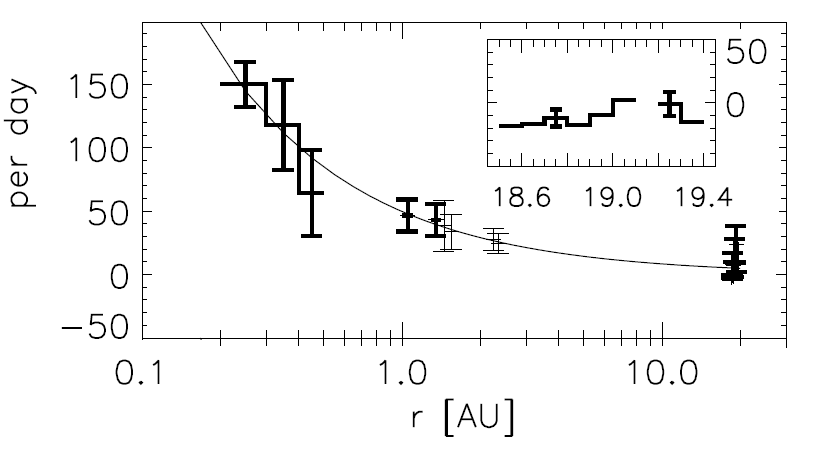
\includegraphics{figures/schematic.png}

}

\caption{\label{fig-1}Distribution of occurrence rate of solar wind discontinuities \citep{sodingRadialLatitudinalDependencies2001}.}

\end{figure}%

\begin{figure}

\centering{

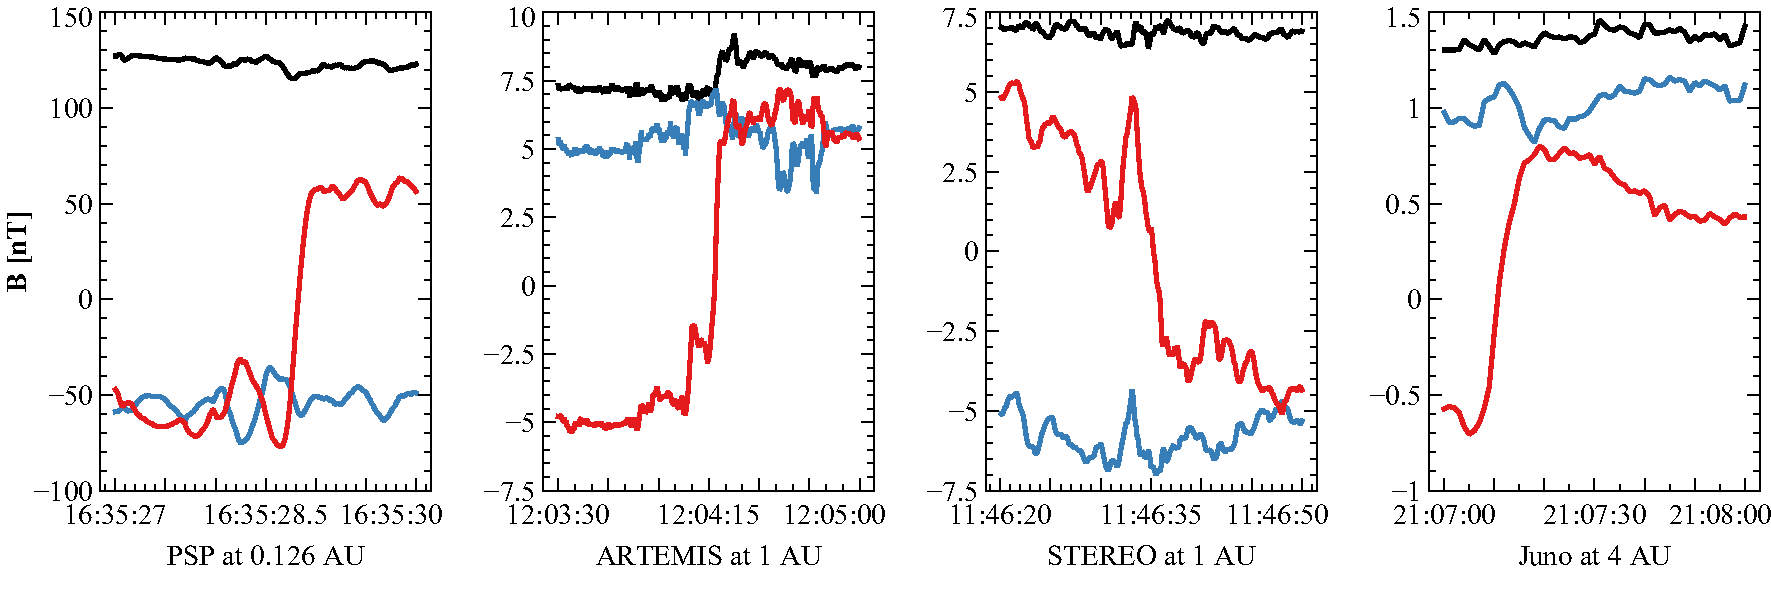
\includegraphics{figures/fig-ids_examples.pdf}

}

\caption{\label{fig-examples}Discontinuities detected by PSP, Juno, STEREO and near-Earth ARTEMIS satellite: red, blue, and black lines are \(B_l\), \(B_m\), and \(|{\mathbf B}|\).}

\end{figure}%

\begin{figure}

\centering{

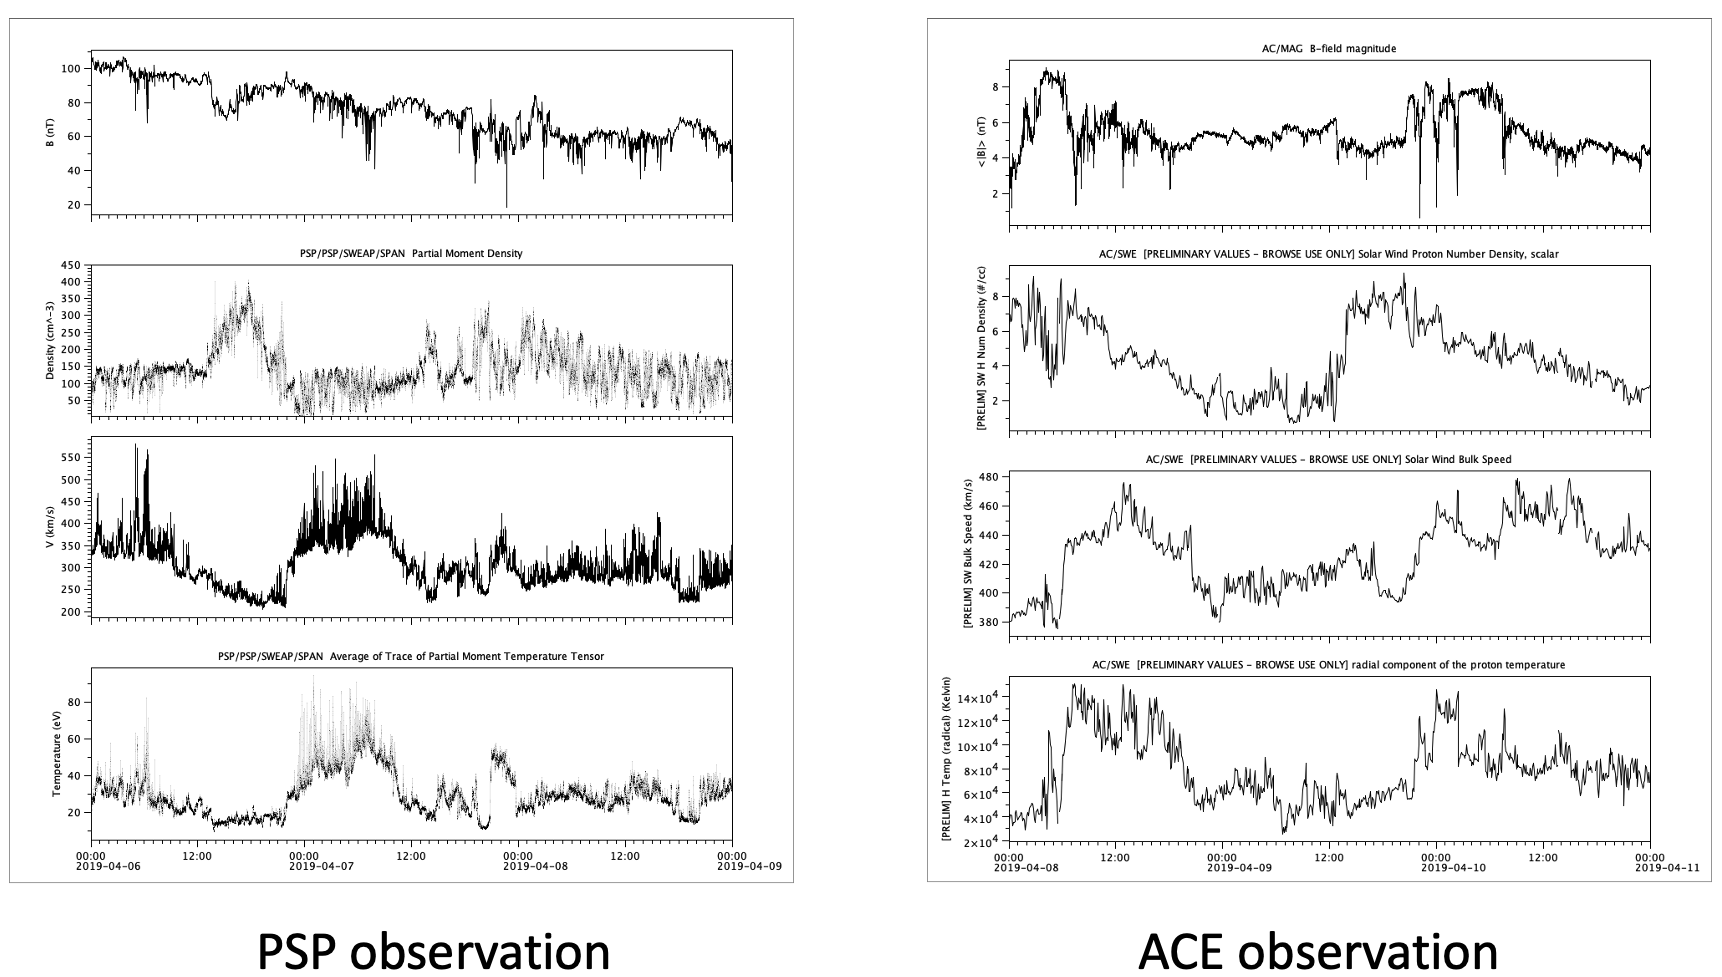
\includegraphics{figures/psp_alignment.png}

}

\caption{\label{fig-alignment}Measurement by PSP and ACE spacecrafts from 2019-04-06 to 2019-04-10. From top to bottom: (a) Magnetic field magnitude measured (b) Plasma density, (c) Plasma velocity, (d) Plasma temperature.}

\end{figure}%

\begin{figure}

\centering{

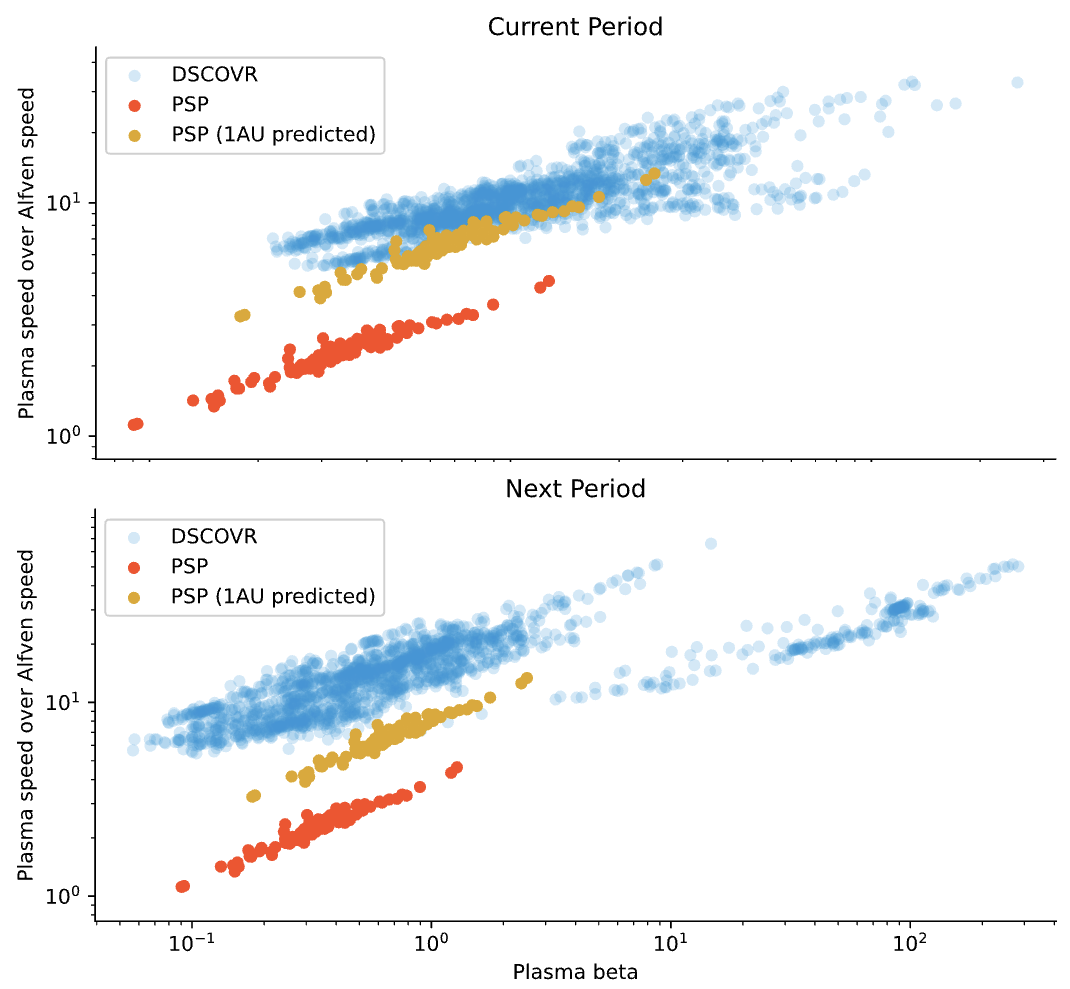
\includegraphics{figures/psp_properties_evolution.png}

}

\caption{\label{fig-evolution}Plasma properties (plasma beta versus plasma speed normalized by Alfven speed) measured by PSP projected to the ACE location using the statistical plasma expansion model. Top panel shows the data from the candidate alignment period (2019-04-06 to 2019-04-07) and the bottom panel shows the data after the alignment period.}

\end{figure}%

\begin{figure}

\centering{

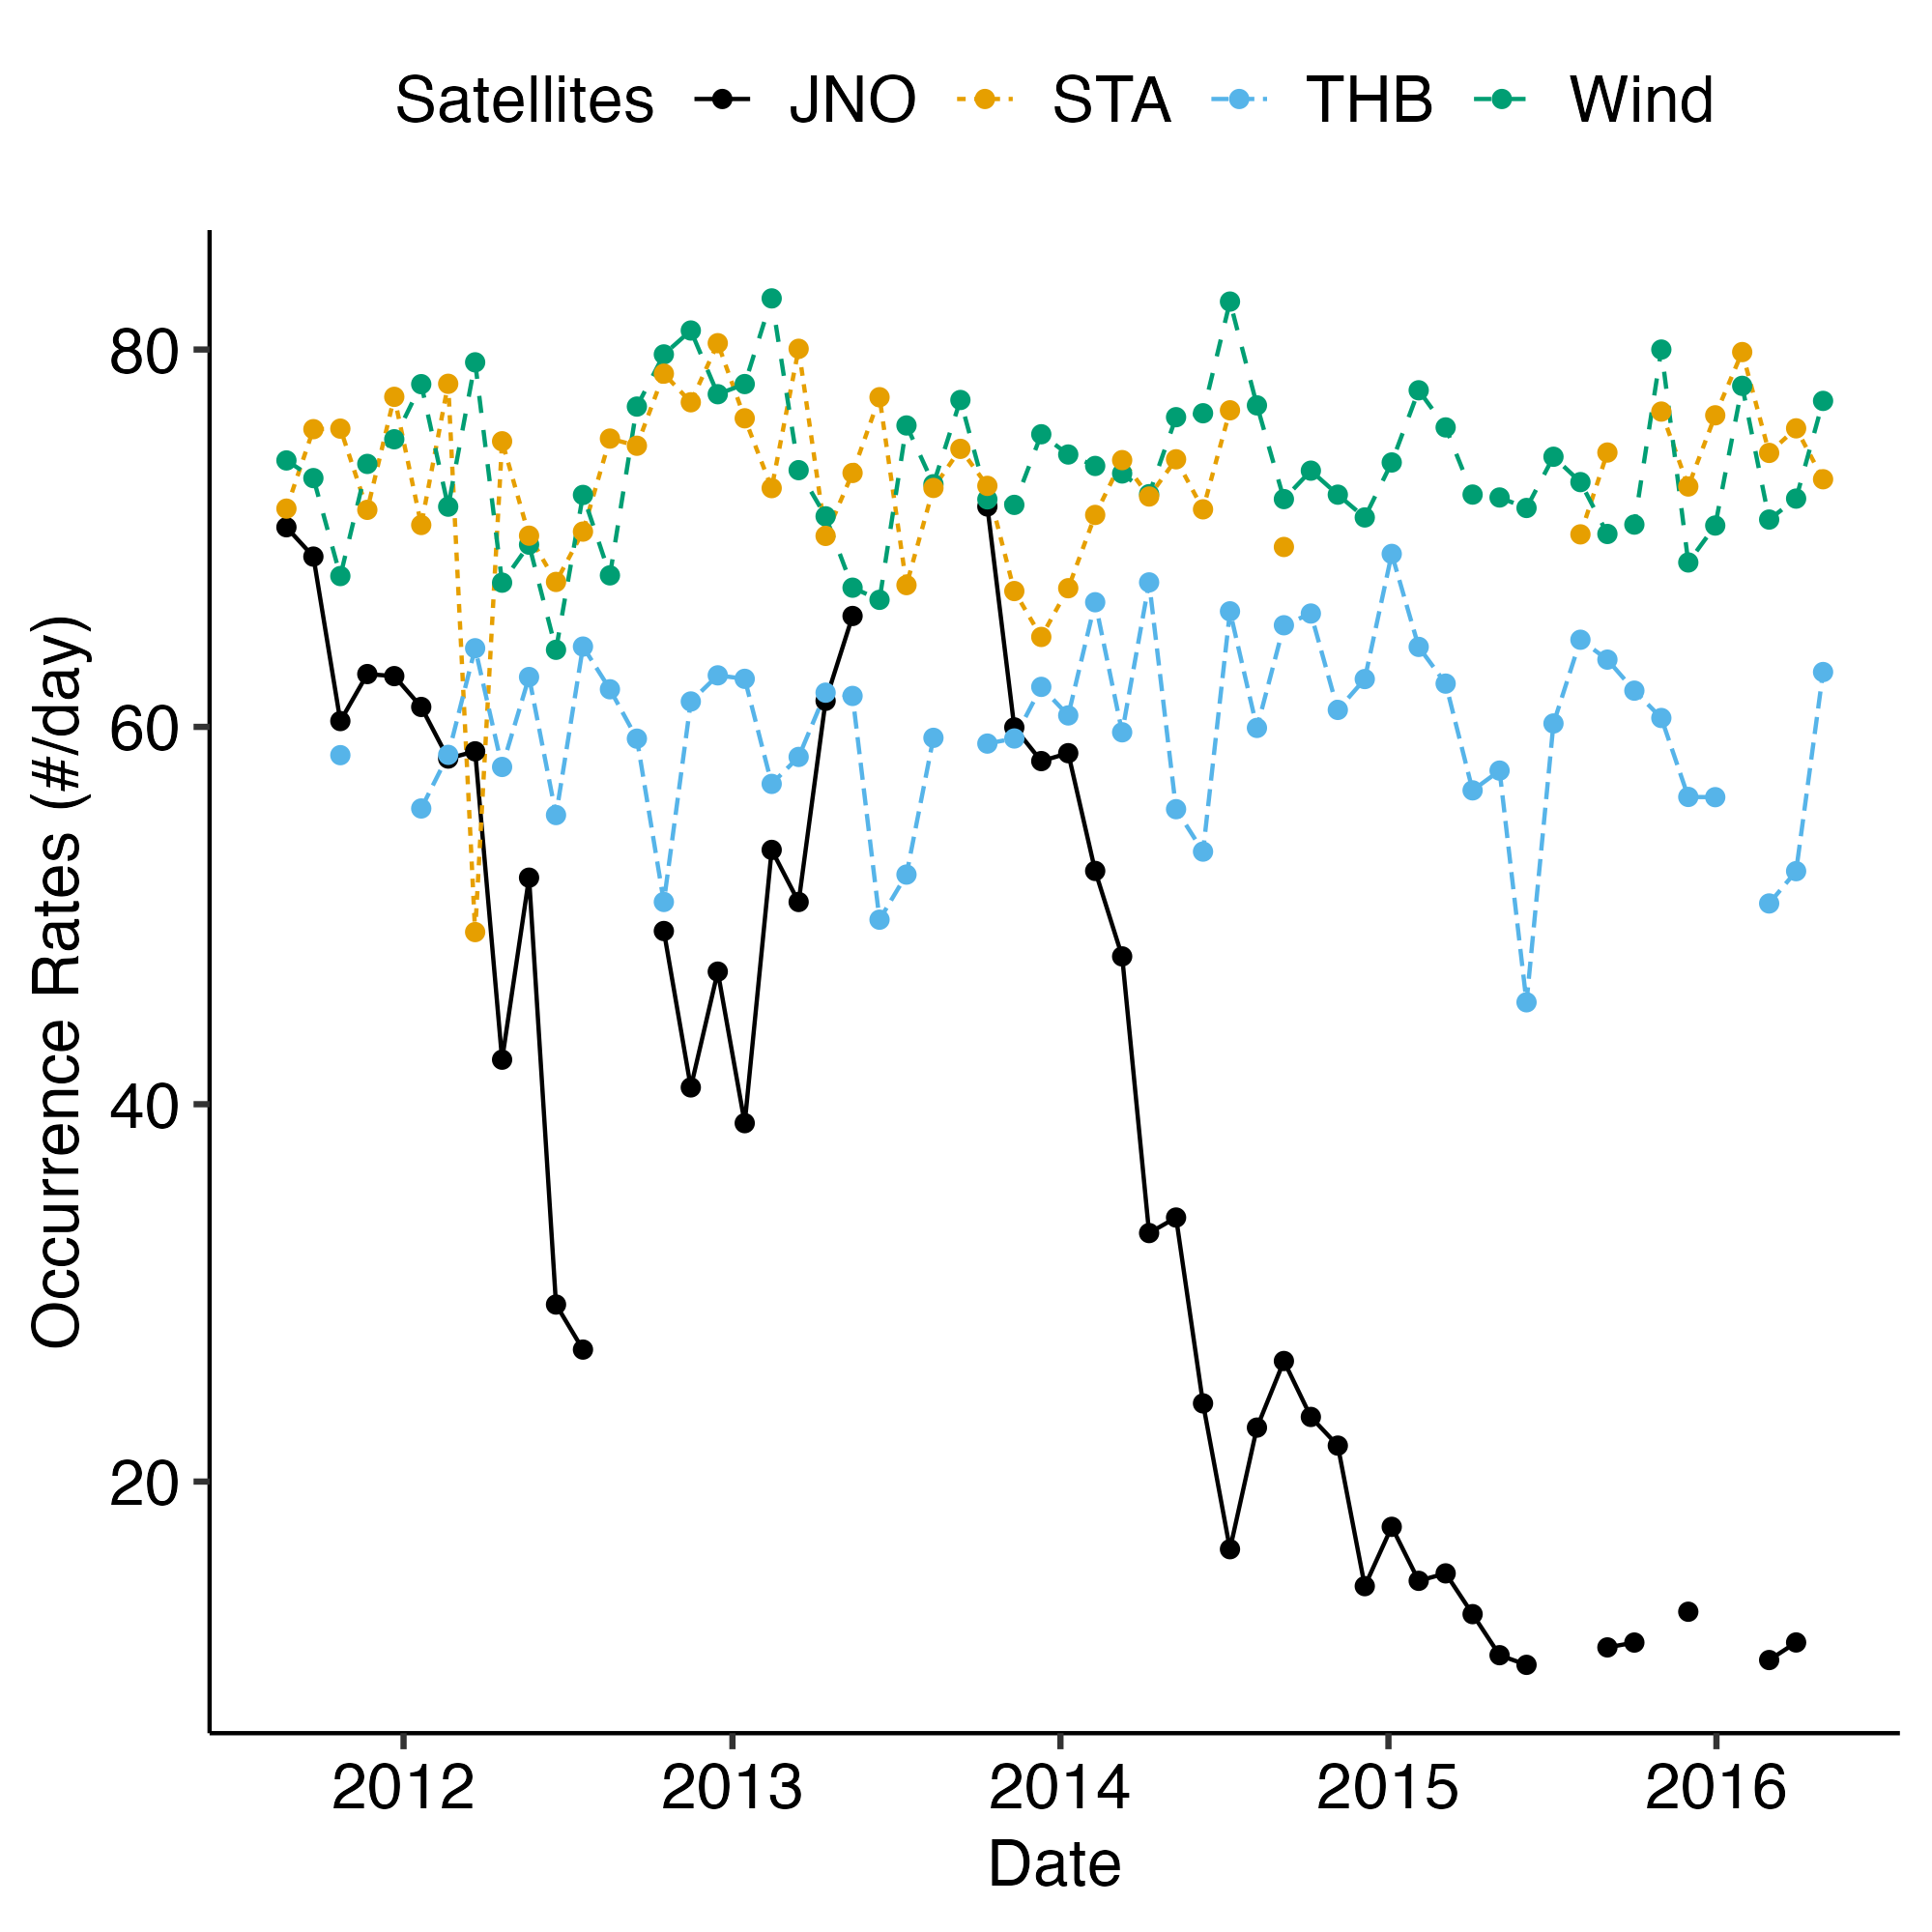
\includegraphics{figures/ocr_time_cleaned.png}

}

\caption{\label{fig-rate}The number of discontinuities measured by Juno per day coincides with the discontinuity number measured by STEREO, WIND, and ARTEMIS, when Juno is around \(1\) AU. This number (occurrence rate) decreases with distance (with time after \(\sim 2013\)), as Juno moves from \(1\) AU to \(5\) AU. We will use the similar comparison for discontinuity characteristics and occurrence rate derived for PSP and Juno.}

\end{figure}%

\begin{figure}

\centering{

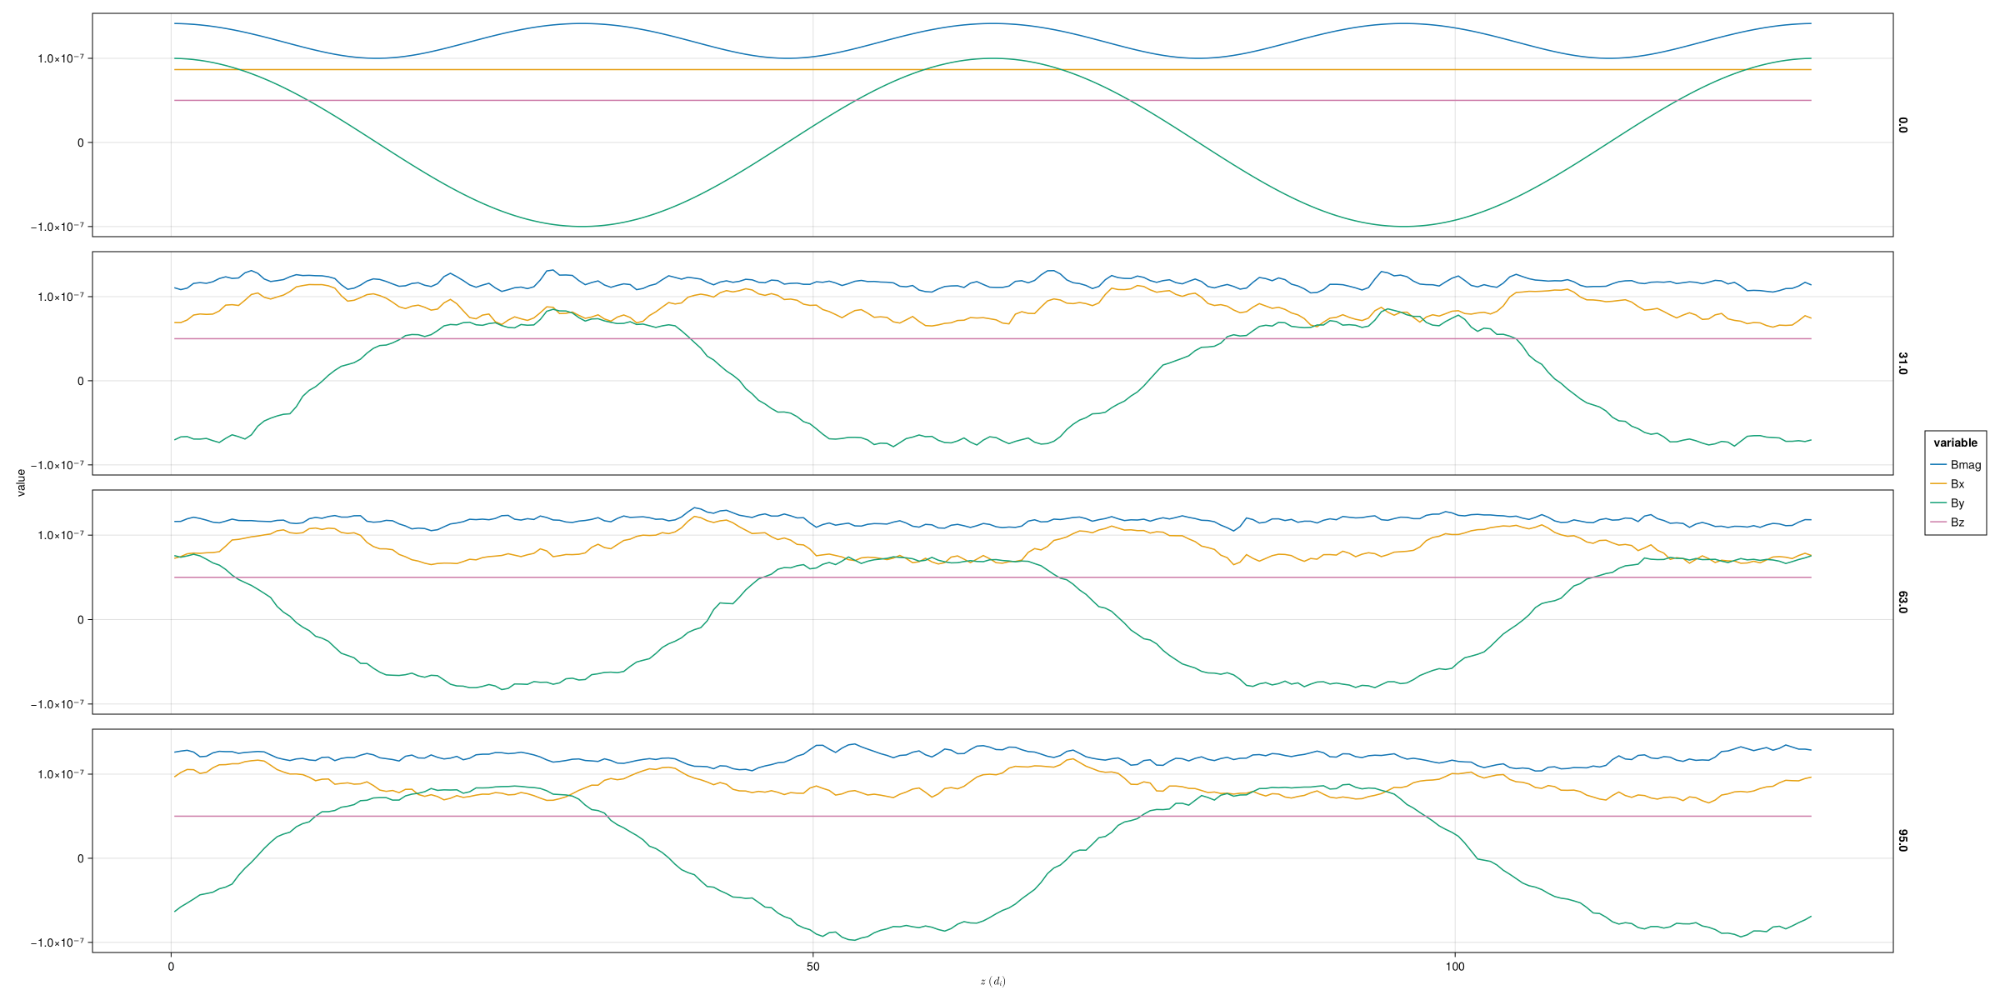
\includegraphics{figures/fig_hybrid.png}

}

\caption{\label{fig-hybrid}Formation of a rotational discontinuity in the solar wind, reproduced using hybrid simulation. The magnetic field components \(B_x\), \(B_y\), \(B_z\), magnetic field magnitude \(|{\mathbf B}|\) are shown in different colors, with each panel corresponding to different times in the simulation normalized by the ion cyclotron period.}

\end{figure}%

\newpage{}


  \bibliography{../../../../files/references.bib,../../../../../share/bibliography/research.bib}


\bibliography{files/Anton.addon.bib,files/Anton.full.bib,files/research.bib}

\end{document}
